\documentclass[tikz]{standalone}
\usepackage{fontspec}
\setmainfont{Futura}
\begin{document}
%
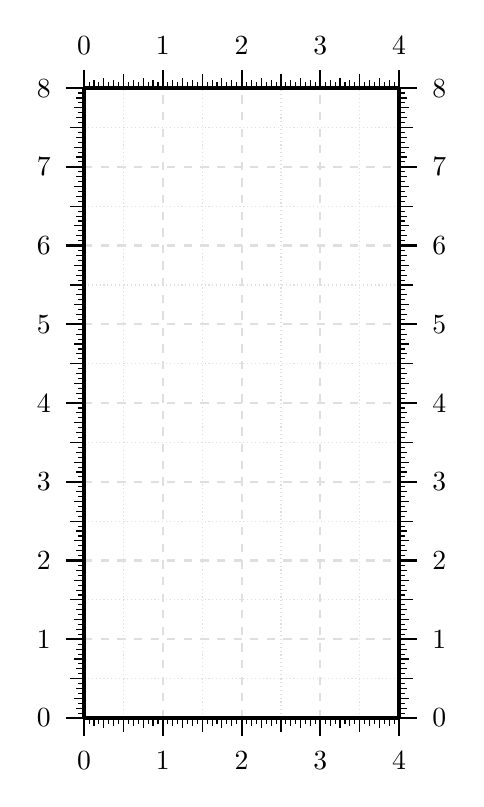
\begin{tikzpicture}
% Draw the grid
\tikzset{help lines/.style={color=gray!25}}
\tikzstyle{EGdensely dotted}=          [dash pattern=on \pgflinewidth off 0.035cm]
\draw[thick,dashed, step=1cm,help lines] (0,0) grid (4,8);
\draw[thin,EGdensely dotted, step=1cm,help lines,xshift=0.5cm,yshift=0.5cm] (0.0,0.0) grid (3.5,7.5);
\draw[thin,EGdensely dotted, step=1cm,help lines,xshift=0.0cm,yshift=0.5cm] (0.0,0.0) grid (0.5,7.5);
\draw[thin,EGdensely dotted, step=1cm,help lines,xshift=0.5cm,yshift=0.0cm] (0.0,0.0) grid (3.5,0.5);
% Draw axes
\draw[ultra thick] (0,0) -- (4,0);
\draw[ultra thick] (4,0) -- (4,8);
\draw[ultra thick] (4,8) -- (0,8);
\draw[ultra thick] (0,8) -- (0,0);

% the co-ordinates -- major
	%bottom
\foreach \x in {0,1,...,4} {     % for x-axis
\draw [thick] (\x,0) -- (\x,-0.225);
}

	%top
\foreach \x in {0,1,...,4} {     % for x-axis
\draw [thick] (\x,8) -- (\x,8.225);
}
	%left
\foreach \y in {0,1,...,8} {   %% for y-axis
\draw [thick] (0,\y) -- (-0.225,\y);
}

	%right
\foreach \y in {0,1,...,8} {   %% for y-axis
\draw [thick] (4,\y) -- (4.225,\y);
}

% the numbers
\foreach \x in {0,1,...,4} { \node [anchor=north] at (\x,-0.3) {\x}; }
\foreach \x in {0,1,...,4} { \node [anchor=south] at (\x,8.3) {\x}; }
\foreach \y in {0,1,...,8} { \node [anchor=east] at (-0.3,\y) {\y}; }
\foreach \y in {0,1,...,8} { \node [anchor=west] at (4.3,\y) {\y}; }

% the co-ordinates --half step
	%bottom
\foreach \x in {.5,1.5,...,3.5} {
\draw [thin] (\x,0) -- (\x,-0.175);
}
	%top
\foreach \x in {.5,1.5,...,3.5} {
\draw [thin] (\x,8) -- (\x,8.175);
}
	%left
\foreach \y in {.5,1.5,...,7.5} {
\draw [thin] (0,\y) -- (-0.175,\y);
}
	%right
\foreach \y in {.5,1.5,...,7.5} {
\draw [thin] (4,\y) -- (4.175,\y);
}

% the co-ordinates --quarter step
	%bottom
\foreach \x in {.25,.5,...,3.75} {
\draw [thin] (\x,0) -- (\x,-0.125);
}
	%top
\foreach \x in {.25,.5,...,3.75} {
\draw [thin] (\x,8) -- (\x,8.125);
}
	%left
\foreach \y in {.25,.5,...,7.75} {
\draw [thin] (0,\y) -- (-0.125,\y);
}
	%right
\foreach \y in {.25,.5,...,7.75} {
\draw [thin] (4,\y) -- (4.125,\y);
}

% the co-ordinates --8th step
	%bottom
\foreach \x in {.125,.25,...,3.875} {
\draw [thin] (\x,0) -- (\x,-0.1);
}
	%top
\foreach \x in {.125,.25,...,3.875} {
\draw [thin] (\x,8) -- (\x,8.1);
}
	%left
\foreach \y in {.125,.25,...,7.875} {
\draw [thin] (0,\y) -- (-0.1,\y);
}
	%right
\foreach \y in {.125,.25,...,7.875} {
\draw [thin] (4,\y) -- (4.1,\y);
}

% the co-ordinates --16th step
	%bottom
\foreach \x in {.0625,.125,...,3.9375} {
\draw [thin] (\x,0) -- (\x,-0.075);
}
	%top
\foreach \x in {.0625,.125,...,3.9375} {
\draw [thin] (\x,8) -- (\x,8.075);
}
	%left
\foreach \y in {.0625,.125,...,7.9375} {
\draw [thin] (0,\y) -- (-0.075,\y);
}
	%right
\foreach \y in {.0625,.125,...,7.9375} {
\draw [thin] (4,\y) -- (4.075,\y);
}
\end{tikzpicture}
%
\end{document}